%Anwendungsfalldiagramme
\section{Anwendungsfälle und Aktivitätsdiagramme}
Die folgenden Anwendungsfälle dienen der Veranschaulichung der möglichen Interaktionen mit \softwarename . Der Ablauf dieser Interaktionen wird anhand von Aktivitätsdiagrammen illustriert.

\subsection{Karteninteraktion}

\begin{center}
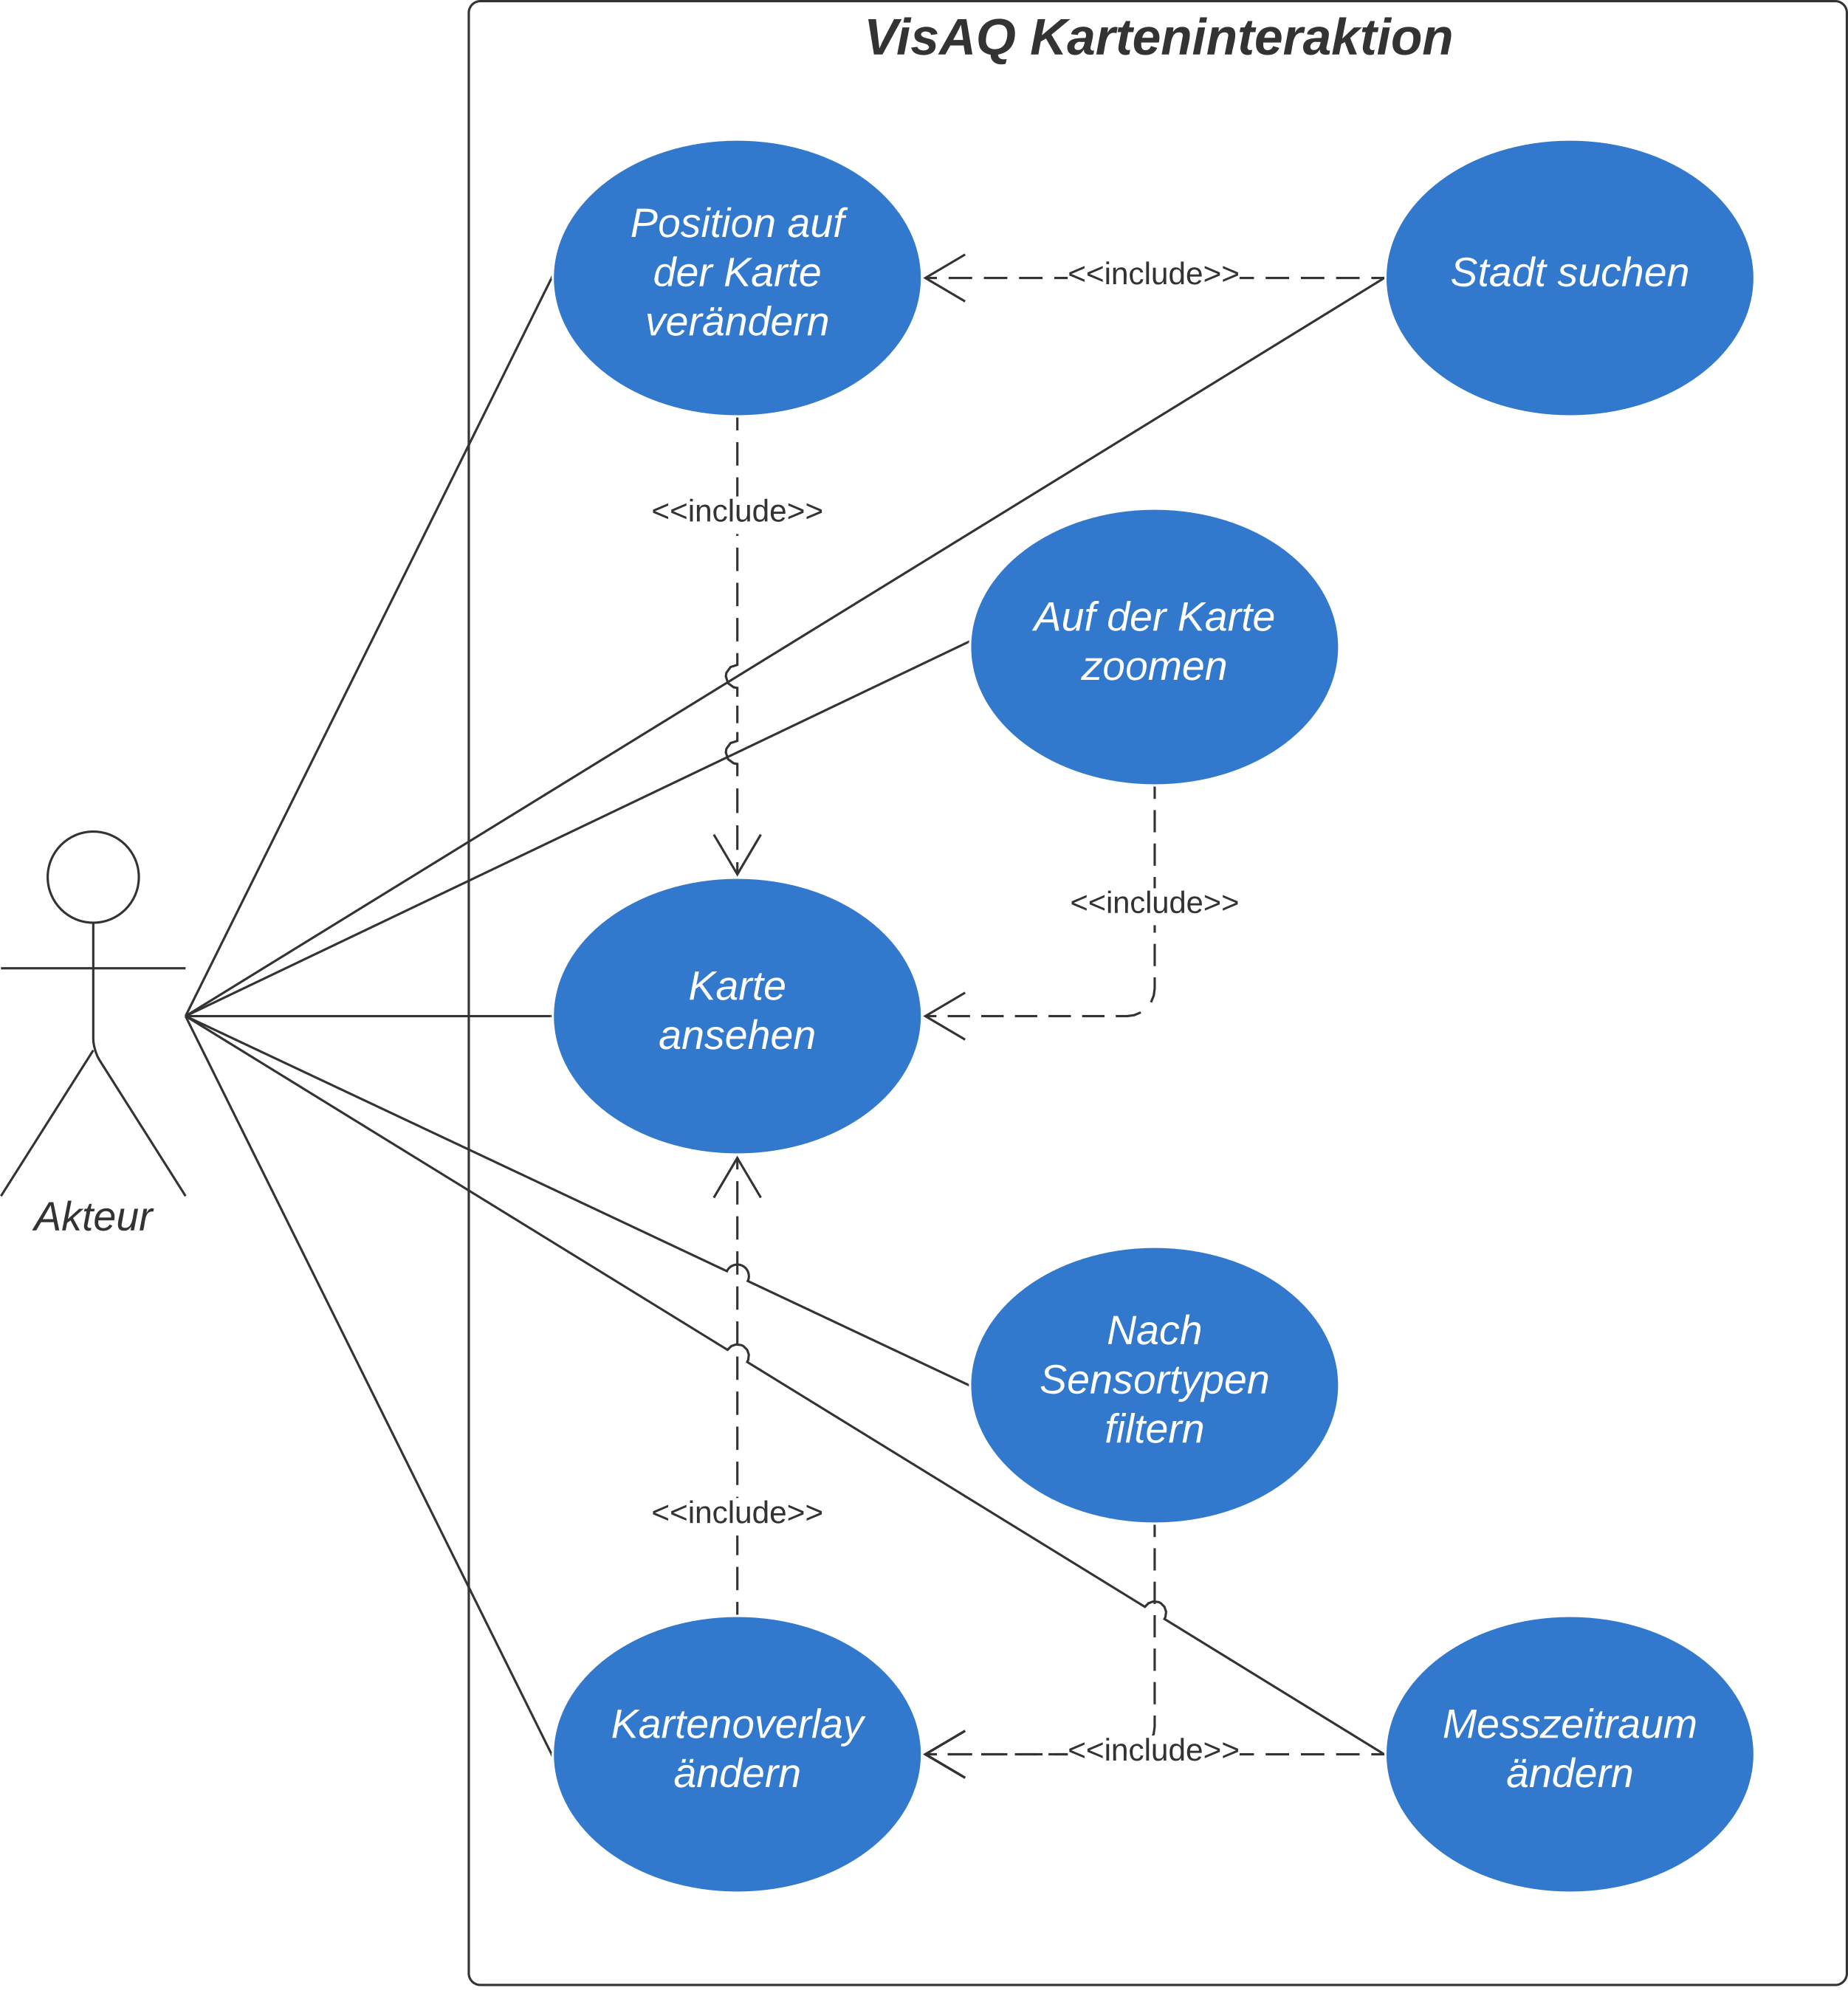
\includegraphics[scale=0.16]{media/activity-usage/Karteninteraktion}\captionof{figure}{Anwendungsfall für die Interaktionen mit der Karte} 

\clearpage

\begin{figure}
\begin{subfigure}[c]{0.5\textwidth}
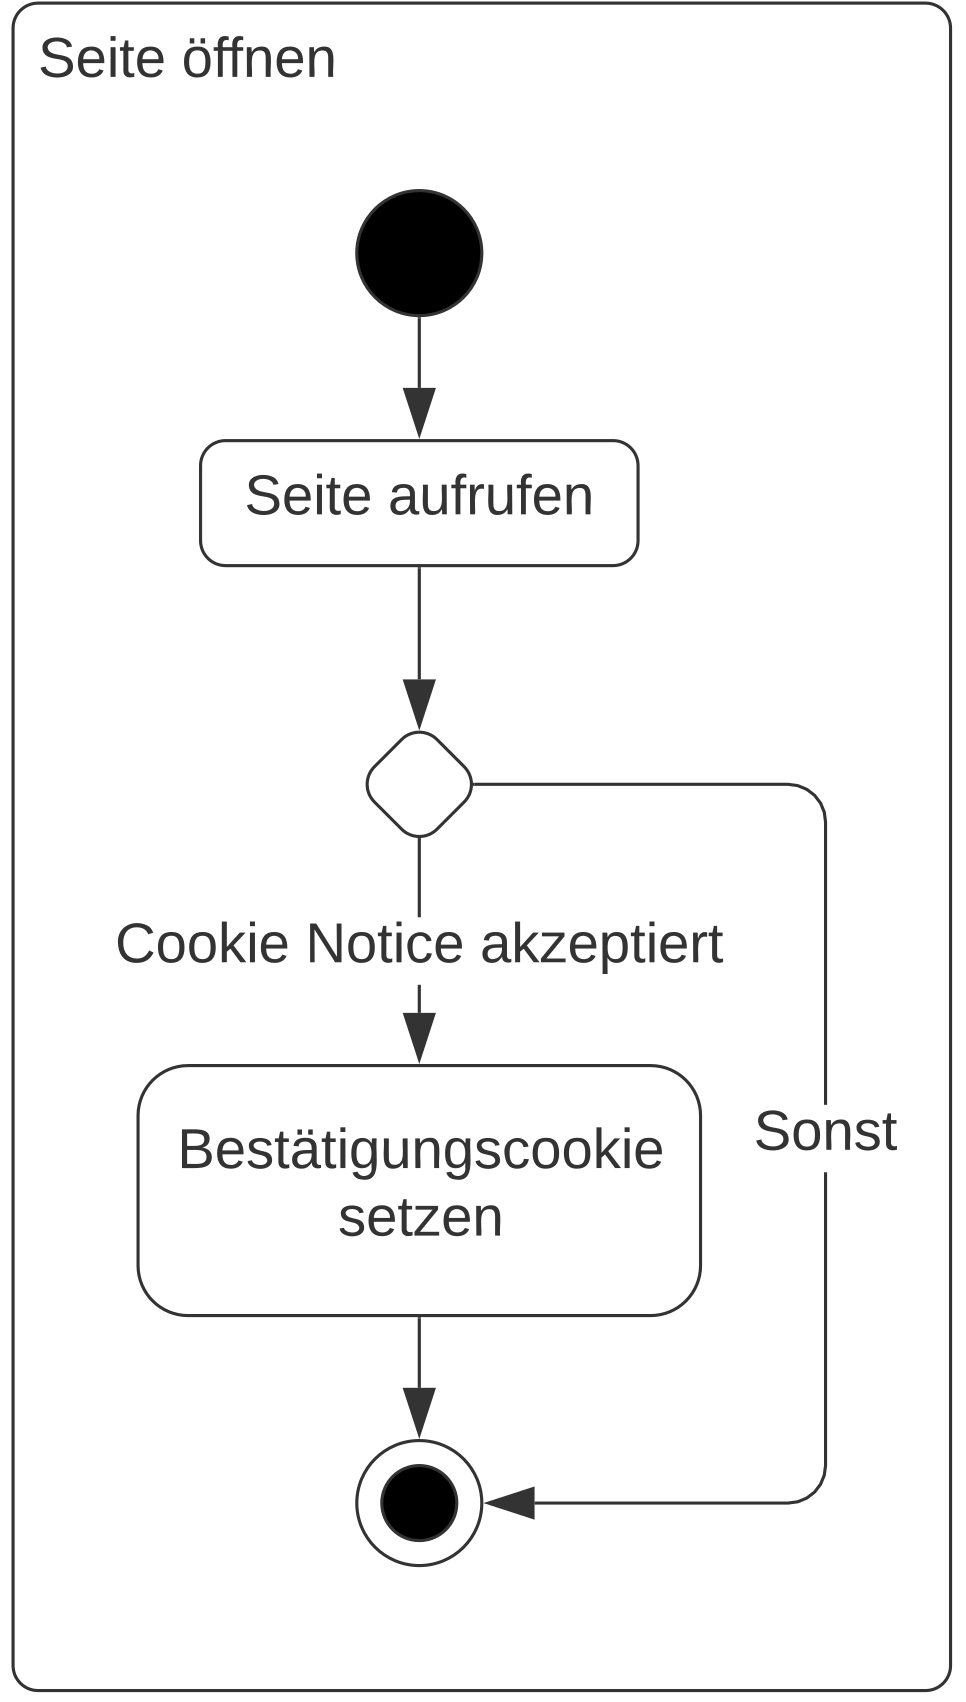
\includegraphics[scale=0.19]{media/activity-usage/SeiteOeffnen}
\end{subfigure}
\begin{subfigure}[c]{0.5\textwidth}
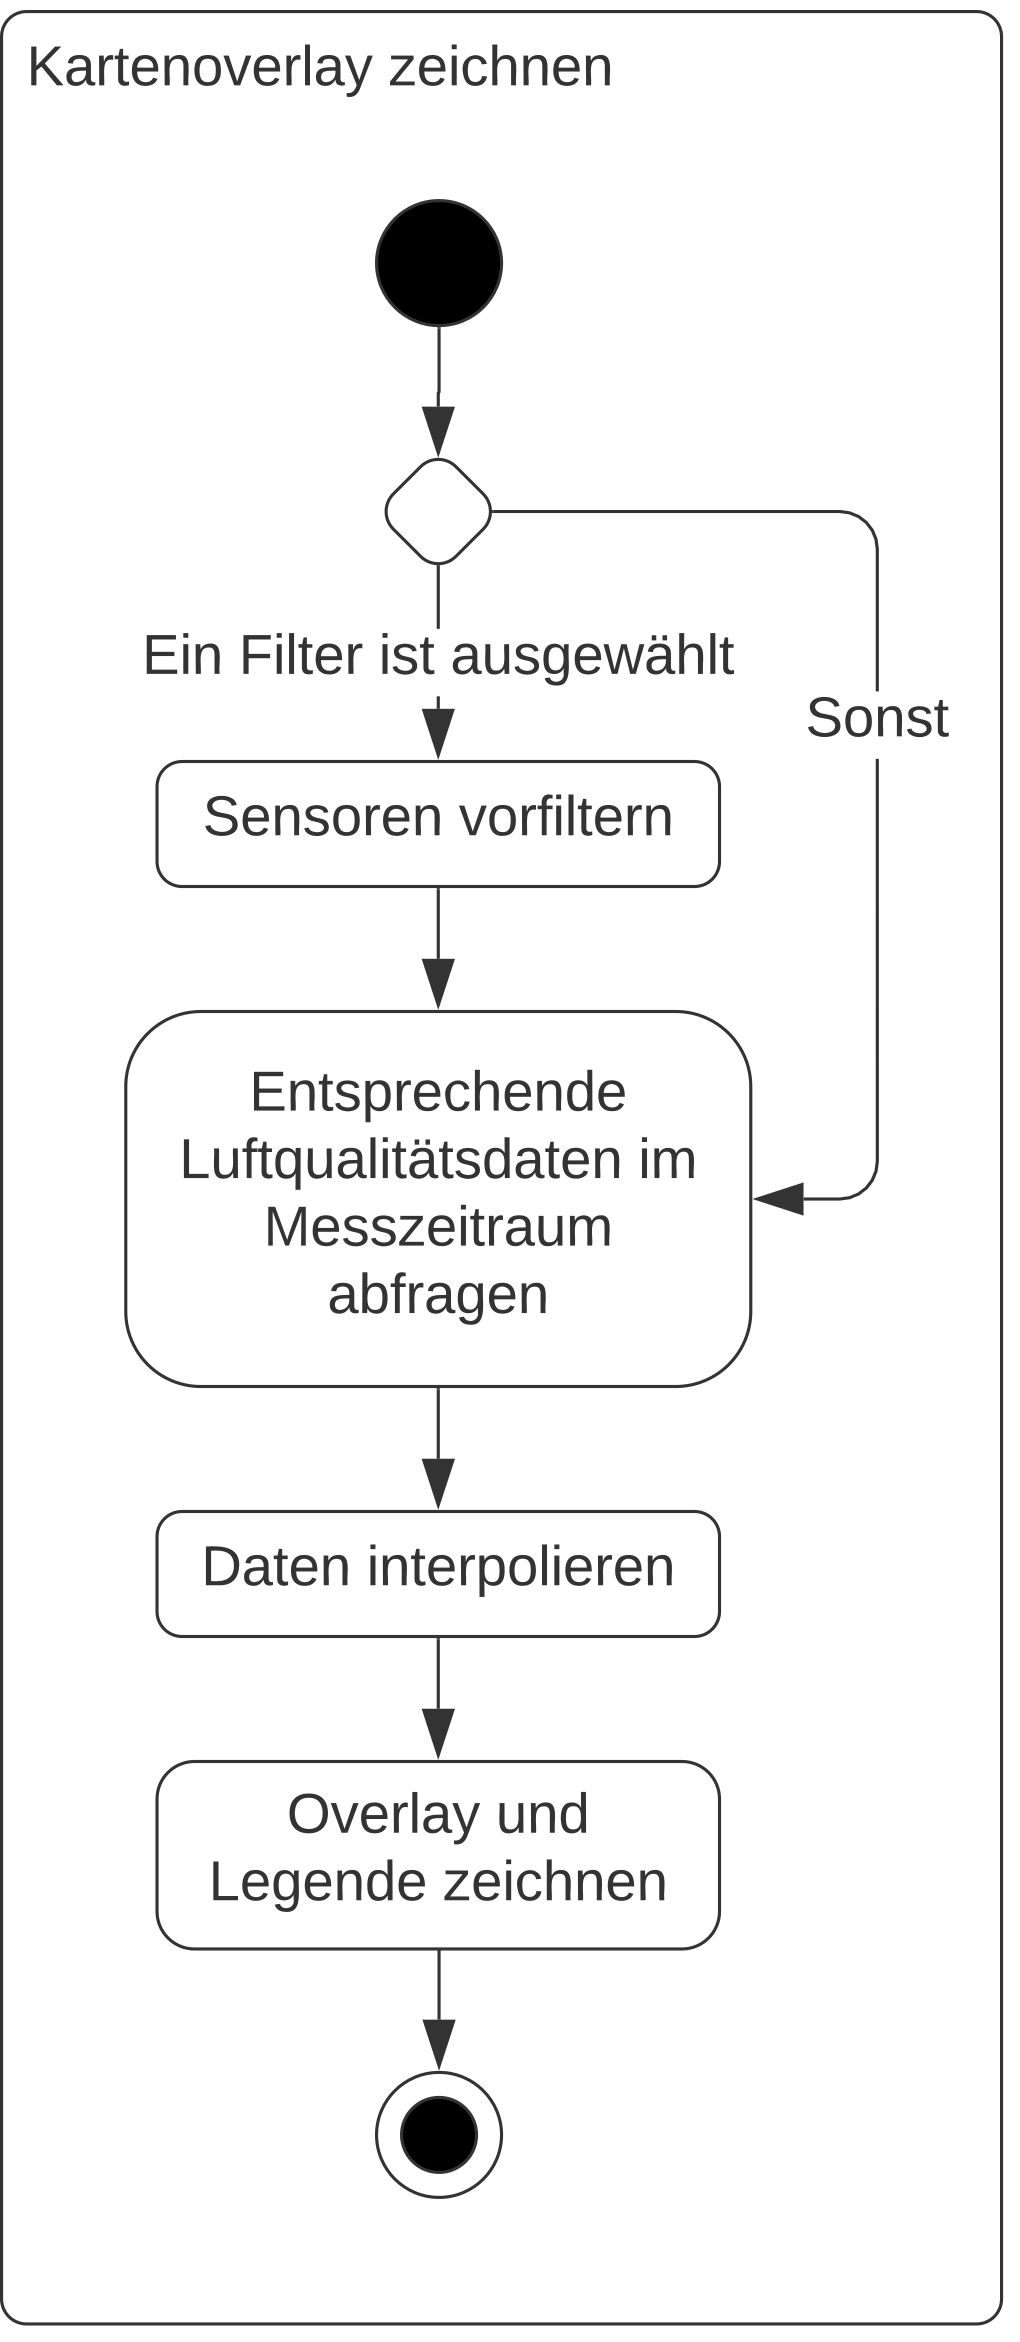
\includegraphics[scale=0.19]{media/activity-usage/KartenoverlayZeichnen}
\end{subfigure}
\caption{Verlauf beim Öffnen der Seite und Zeichnen der Kartenoverlays}
\end{figure}

\clearpage

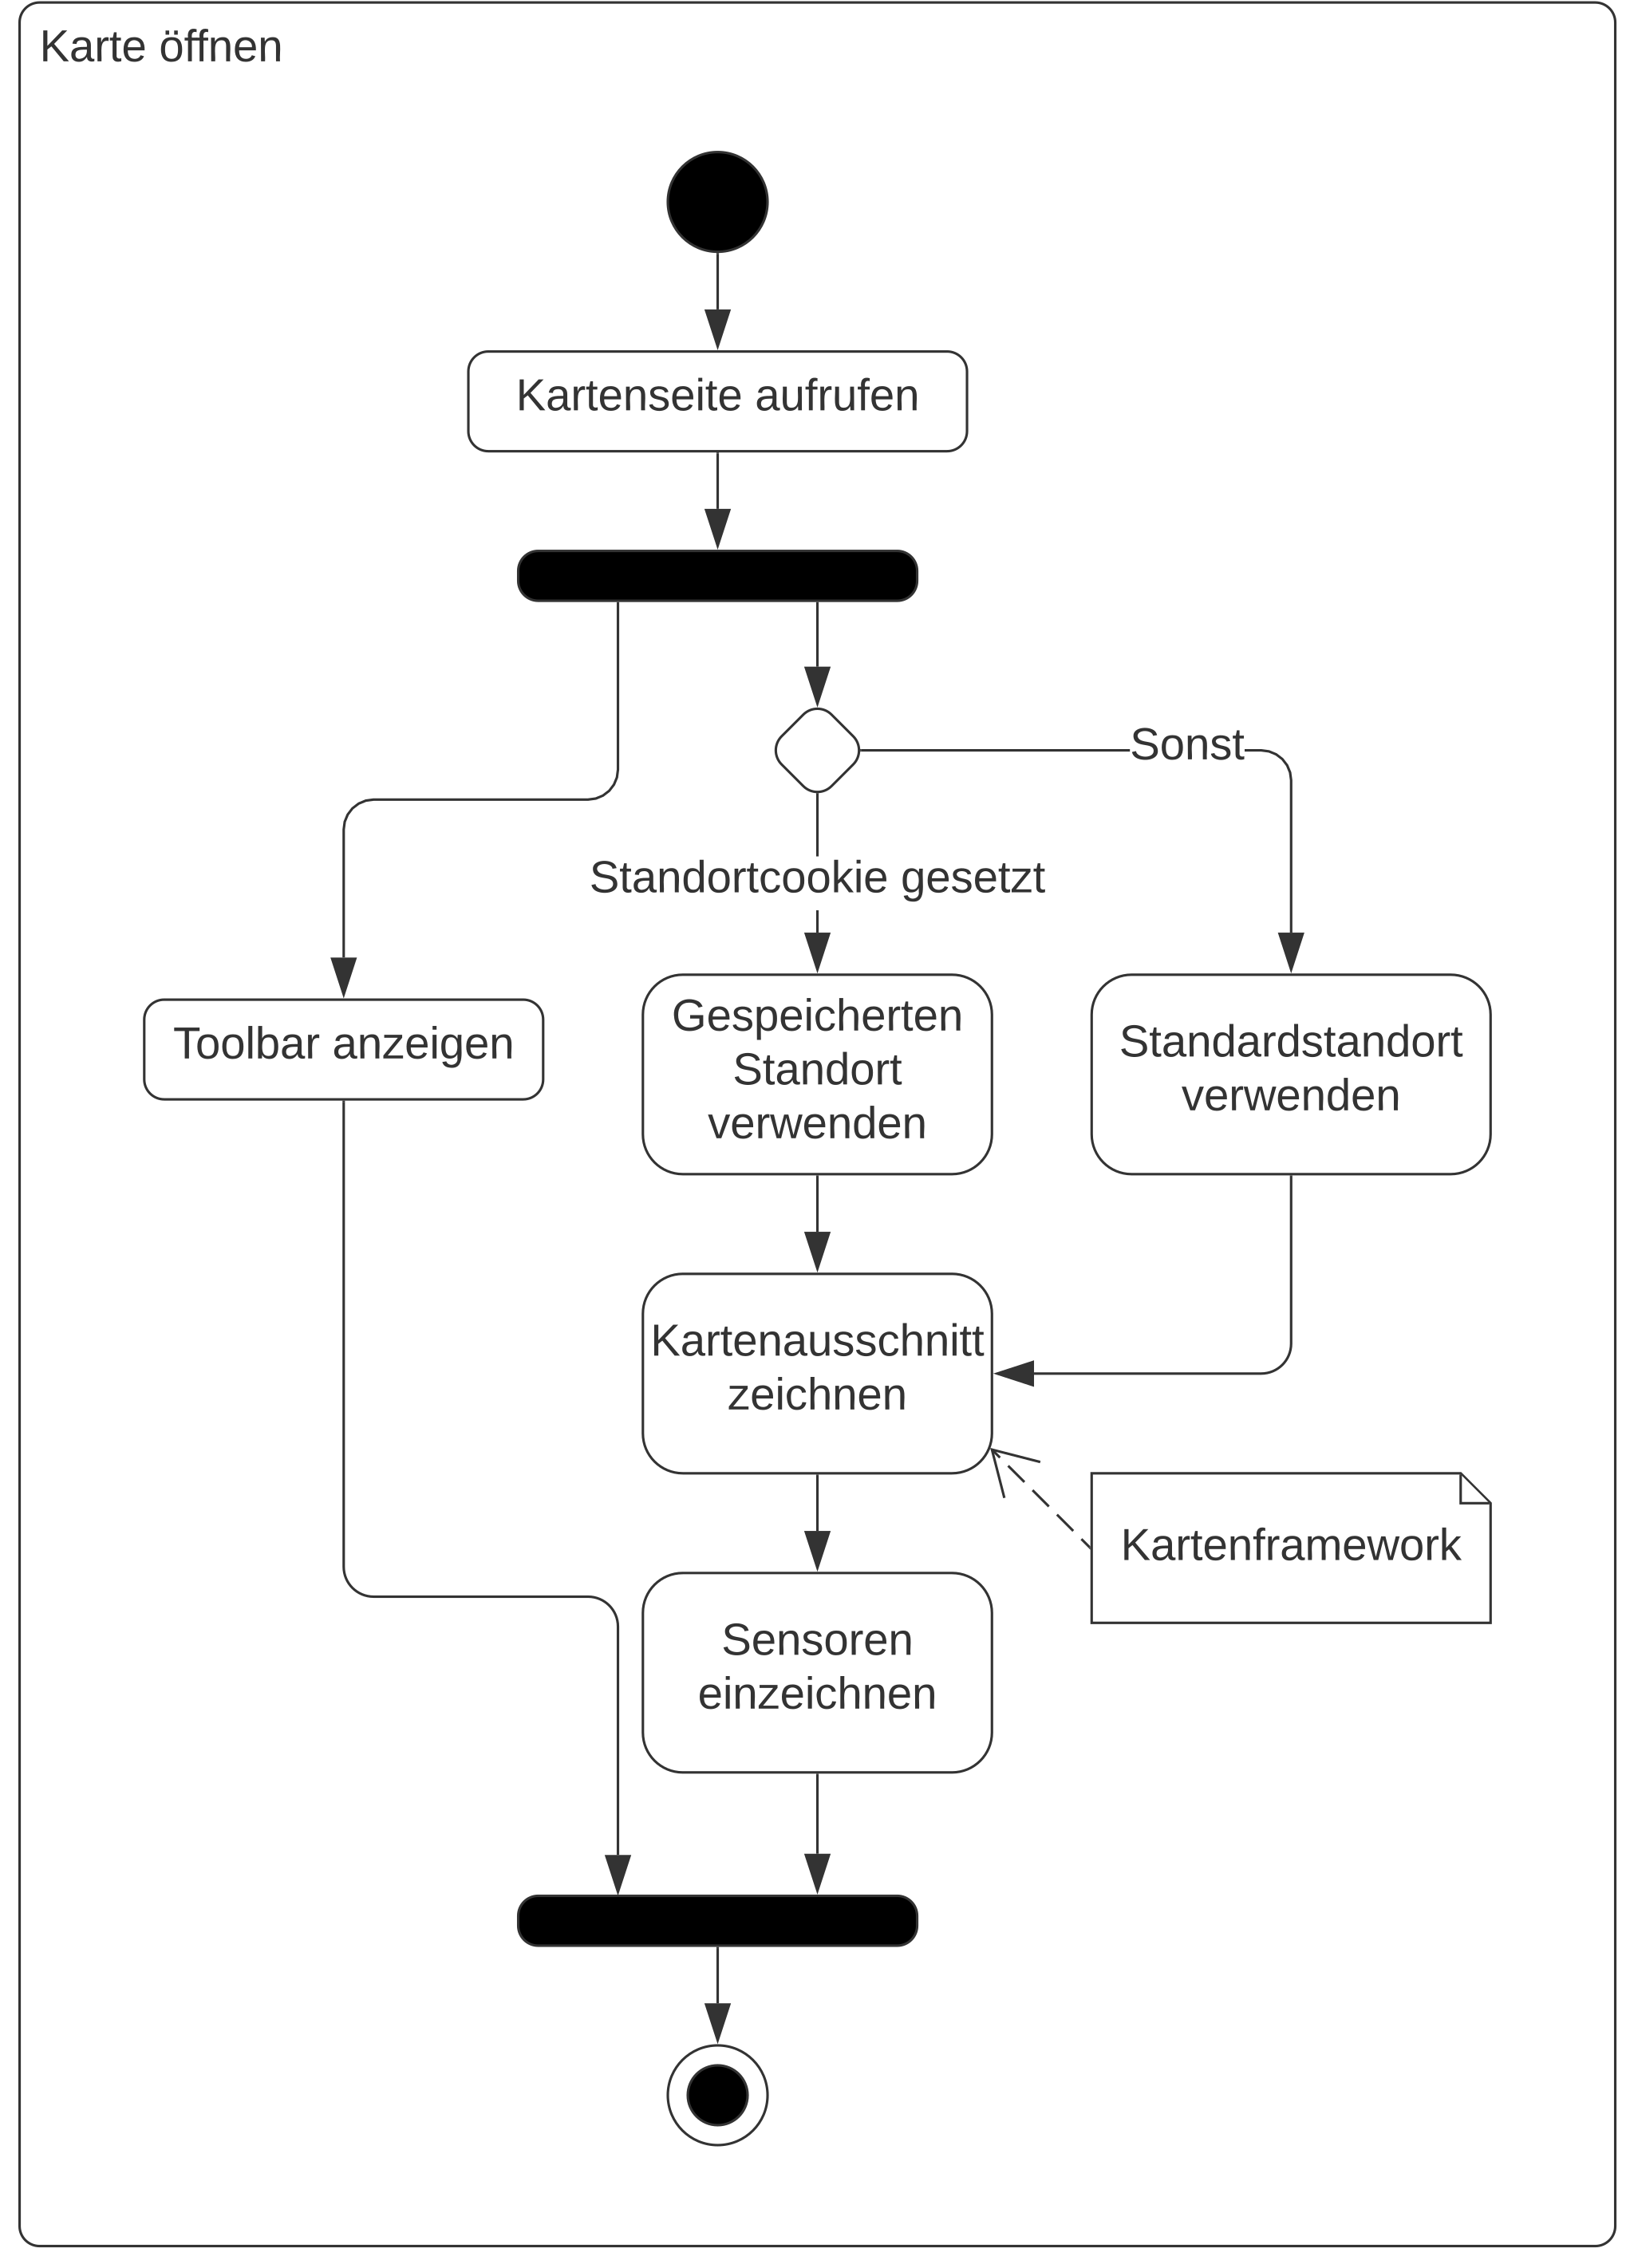
\includegraphics[scale=0.19]{media/activity-usage/KarteOeffnen}\captionof{figure}{Der Ablauf beim Öffnen der Karte} 

\clearpage

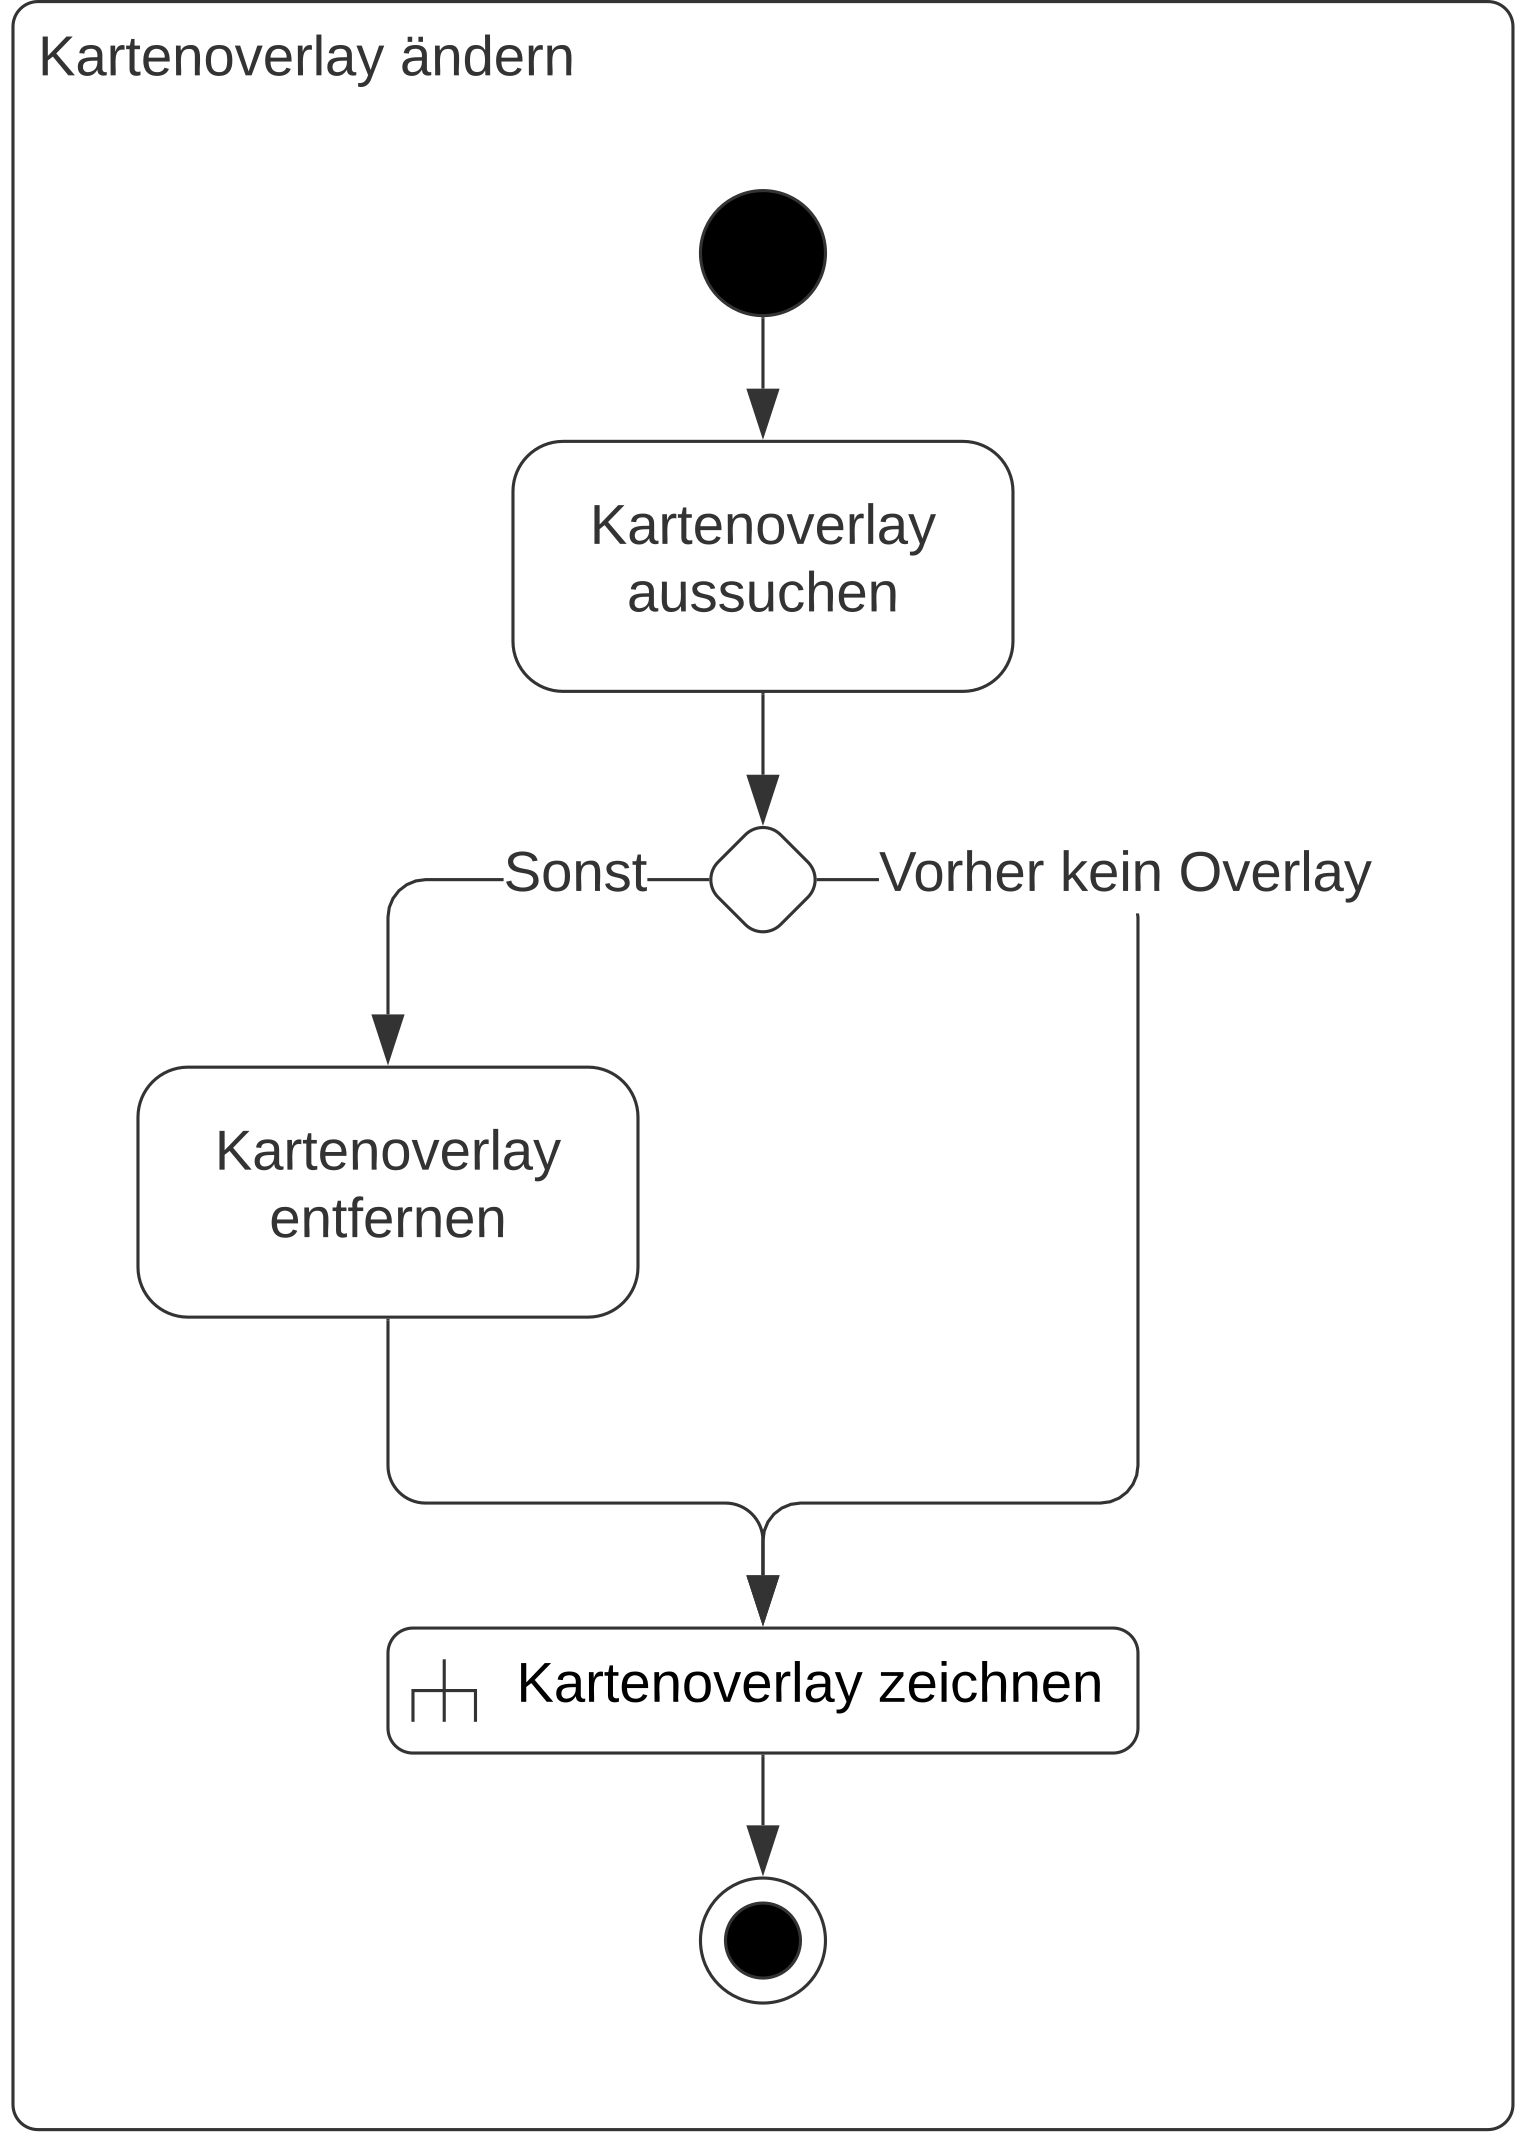
\includegraphics[scale=0.19]{media/activity-usage/KartenoverlayAendern}\captionof{figure}{Verlauf beim Ändern des Kartenoverlays} 

\clearpage

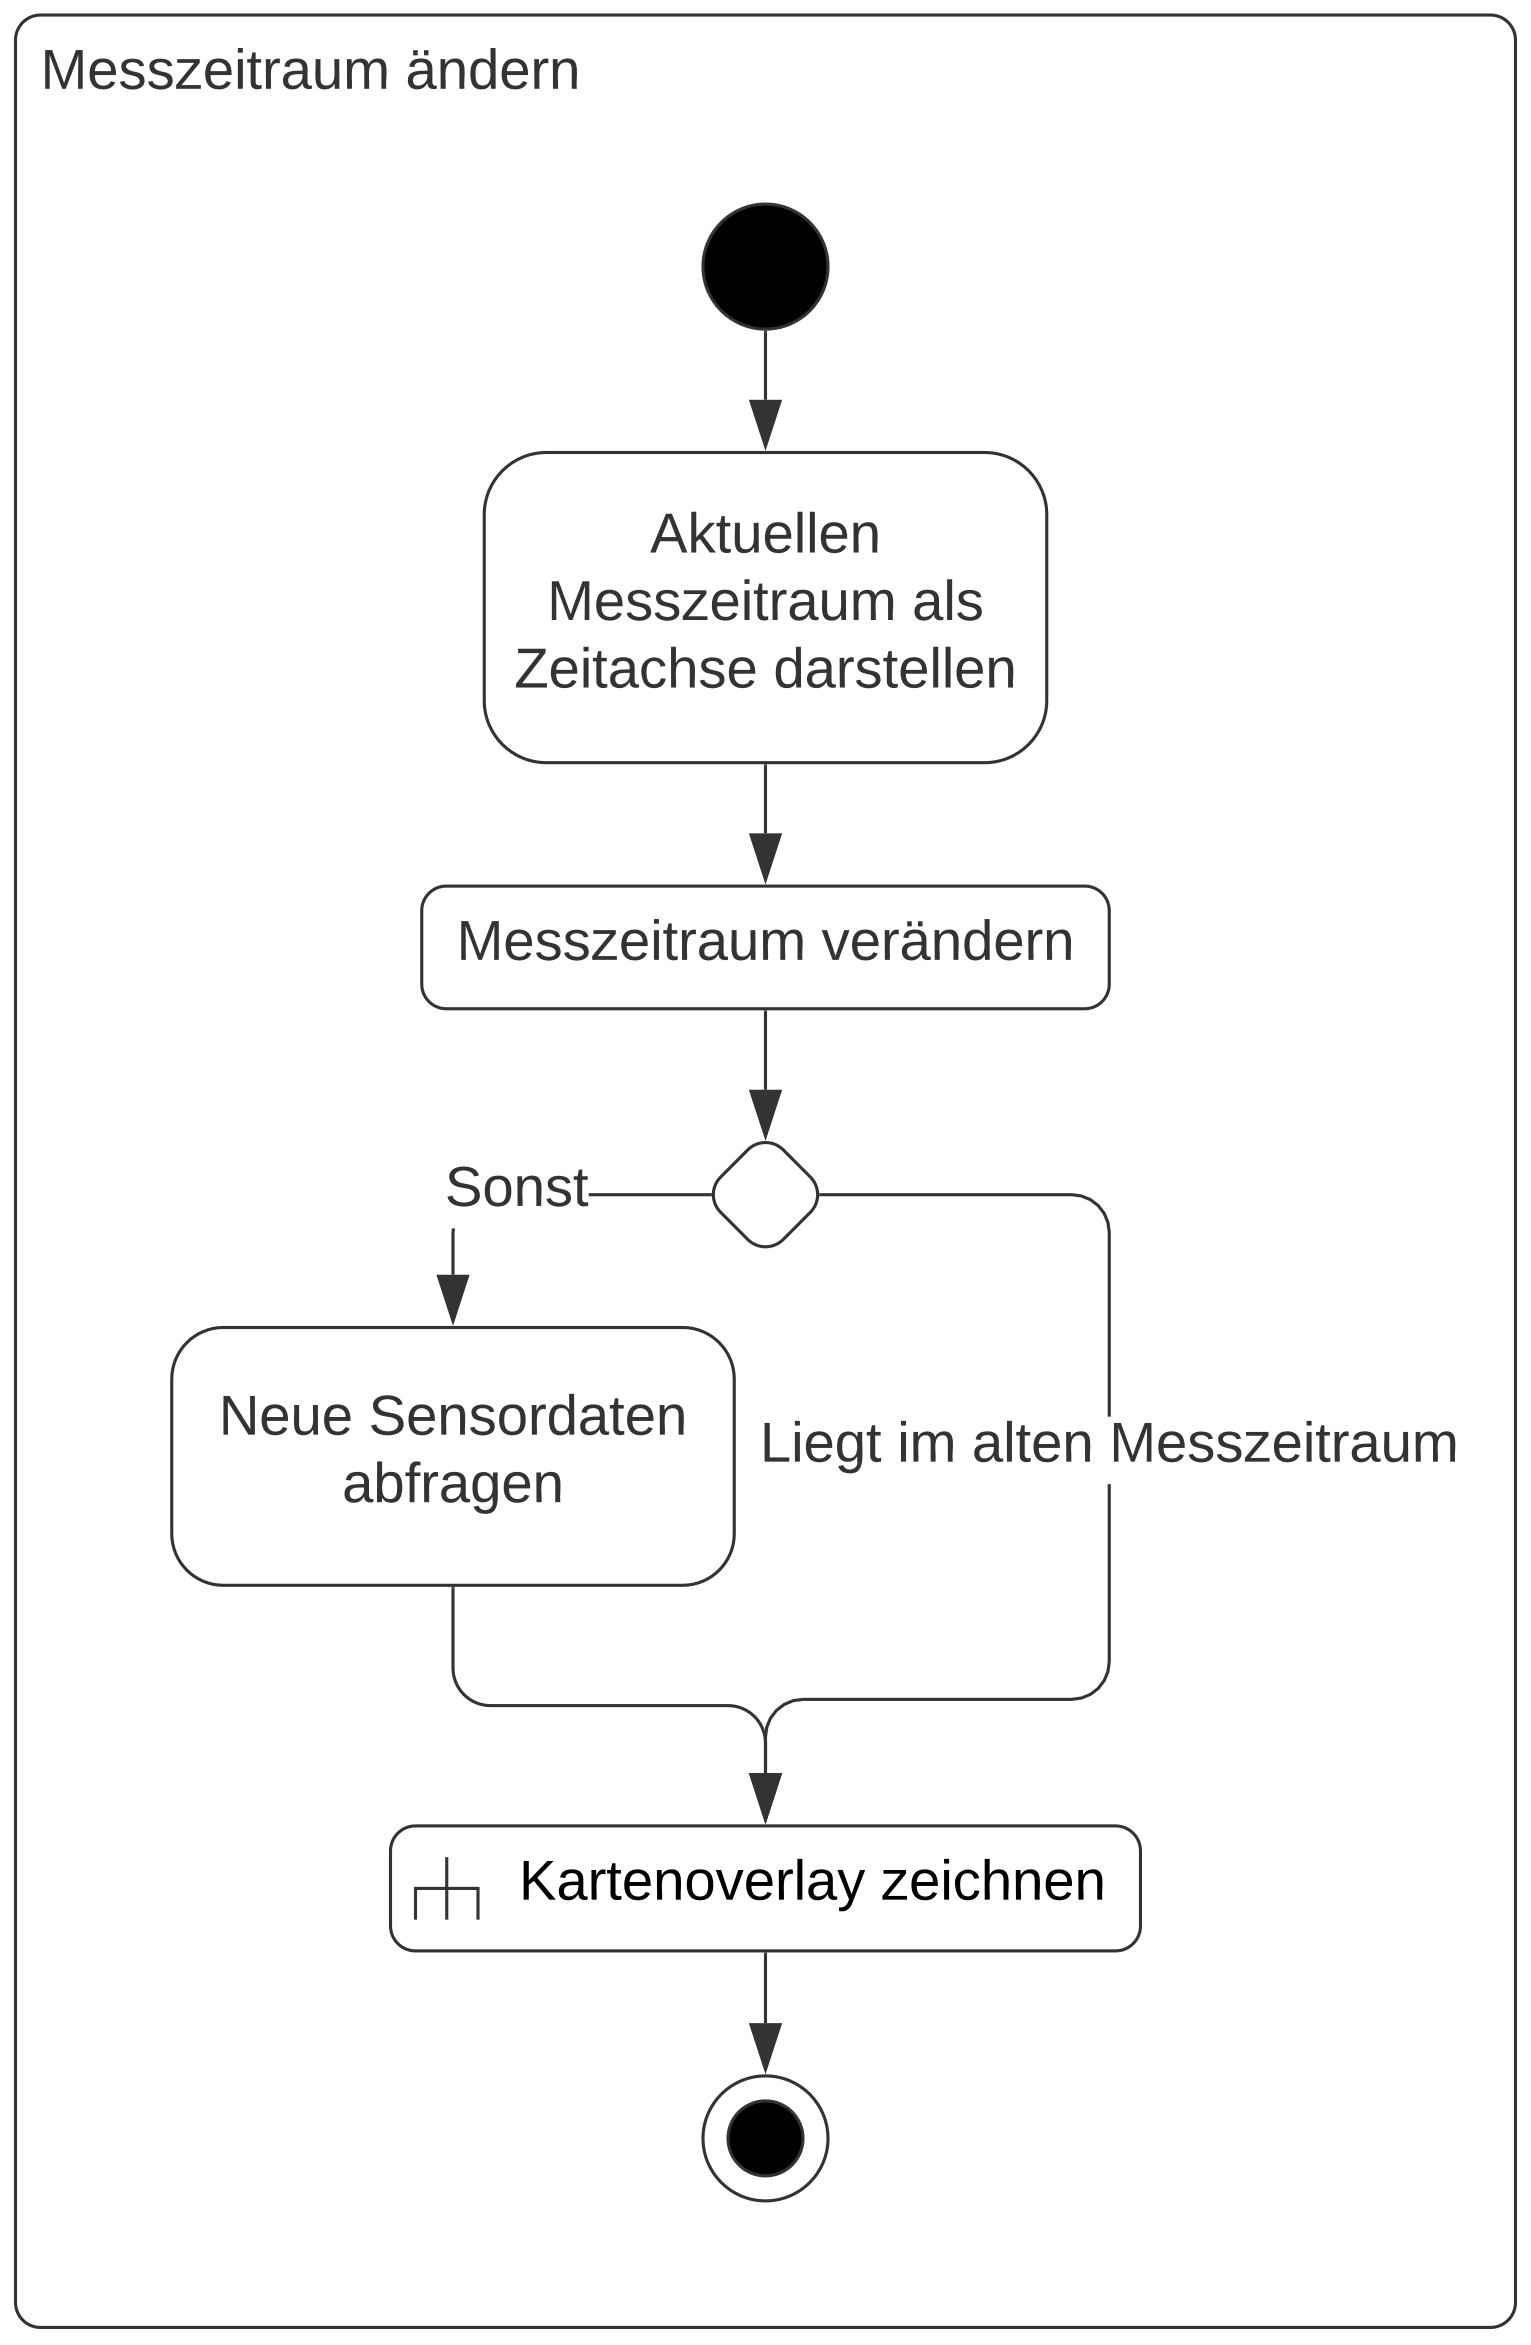
\includegraphics[scale=0.19]{media/activity-usage/MesszeitraumAendern}\captionof{figure}{Das Ändern des Messzeitraums} 

\clearpage

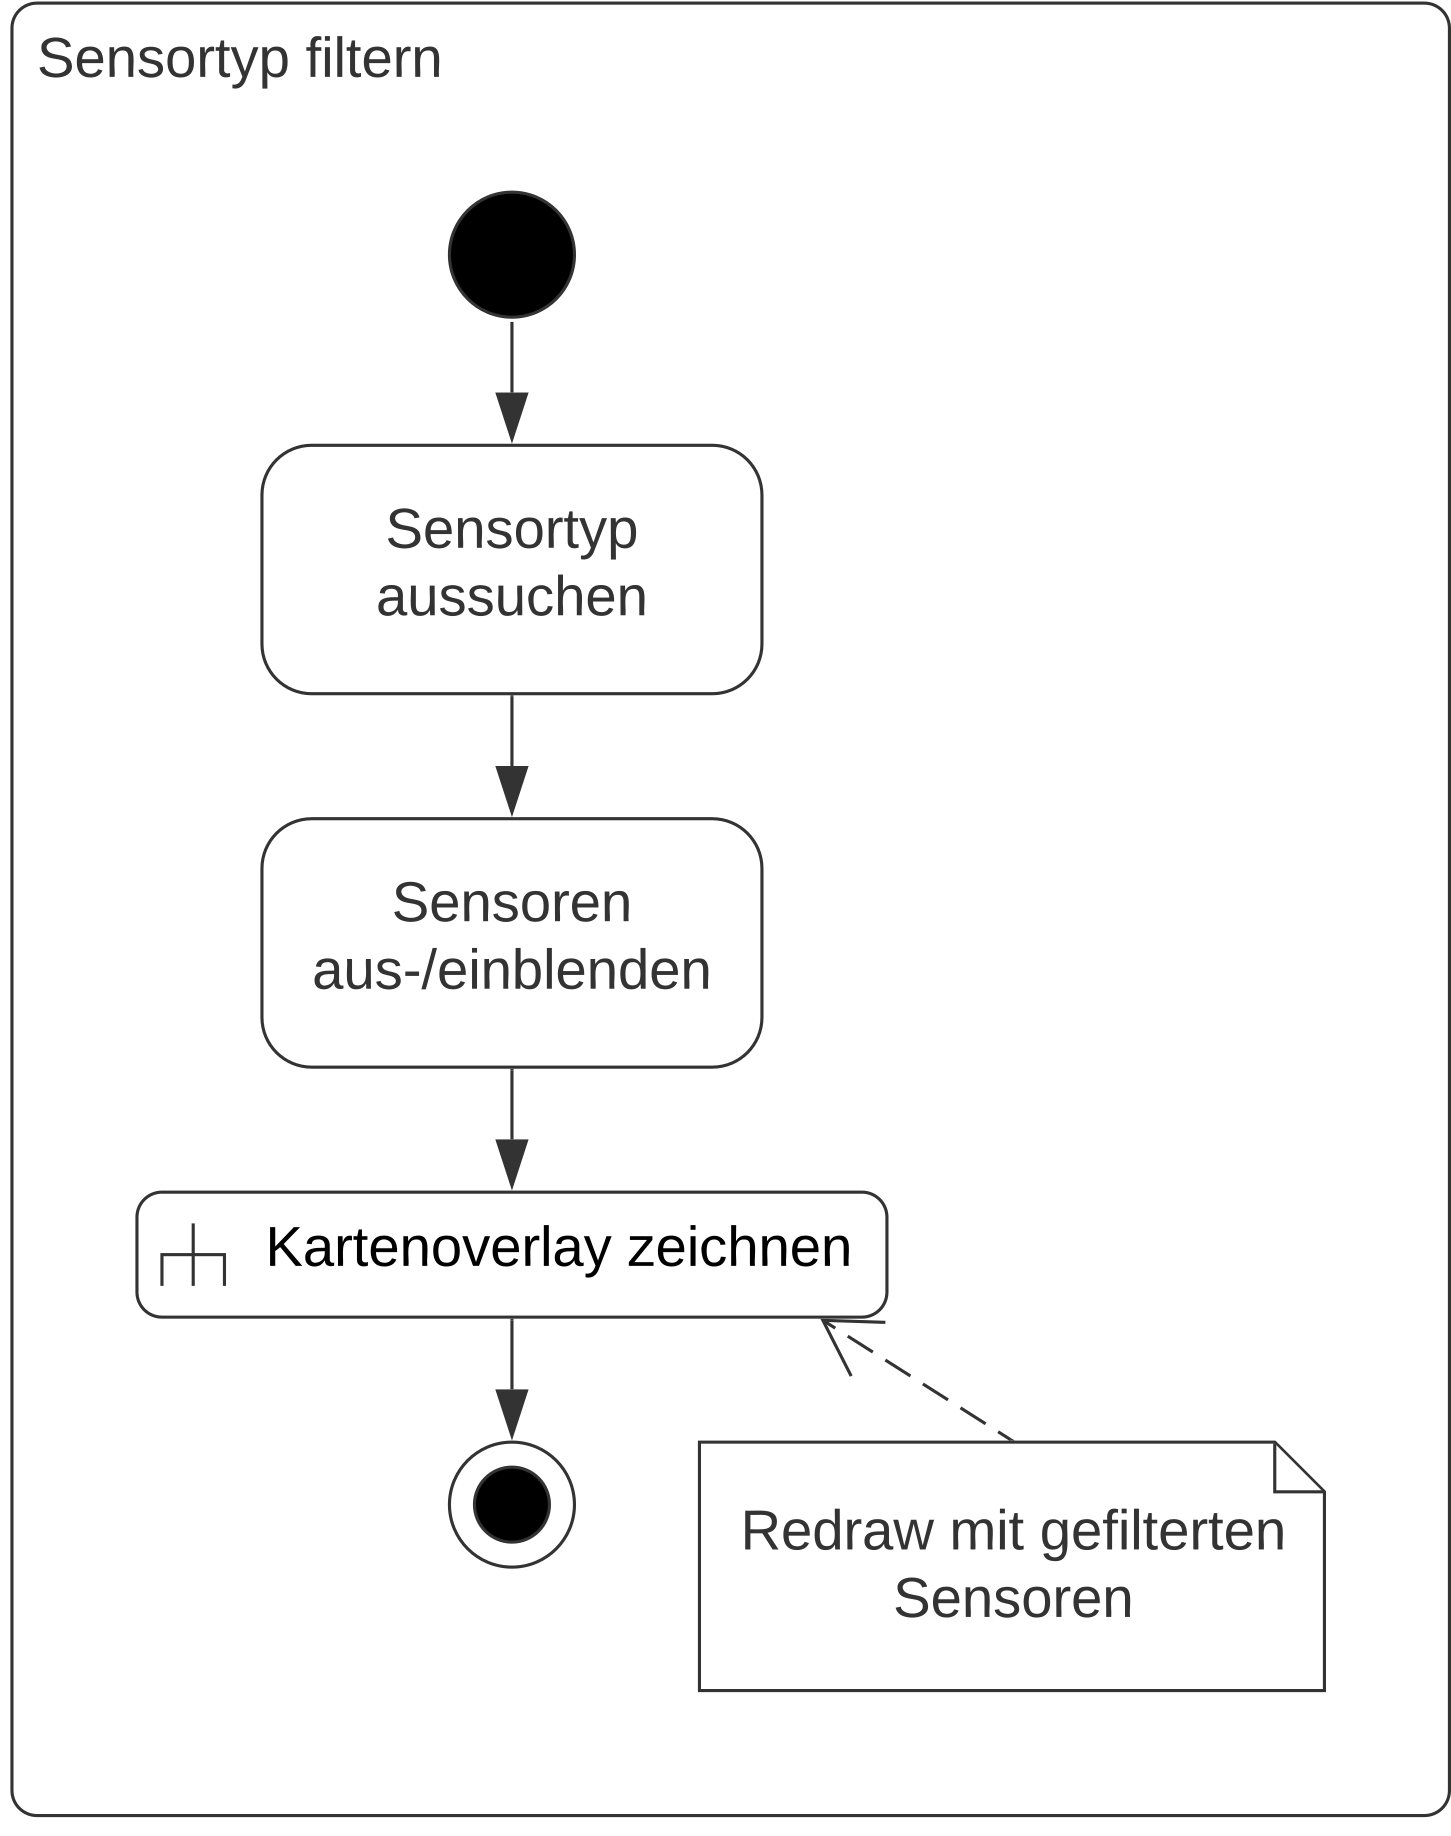
\includegraphics[scale=0.19]{media/activity-usage/SensortypFiltern}\captionof{figure}{Ablauf beim Filtern nach einem Sensortypen}
\end{center}

\clearpage

\subsection{Sensorinteraktion}

\begin{center}
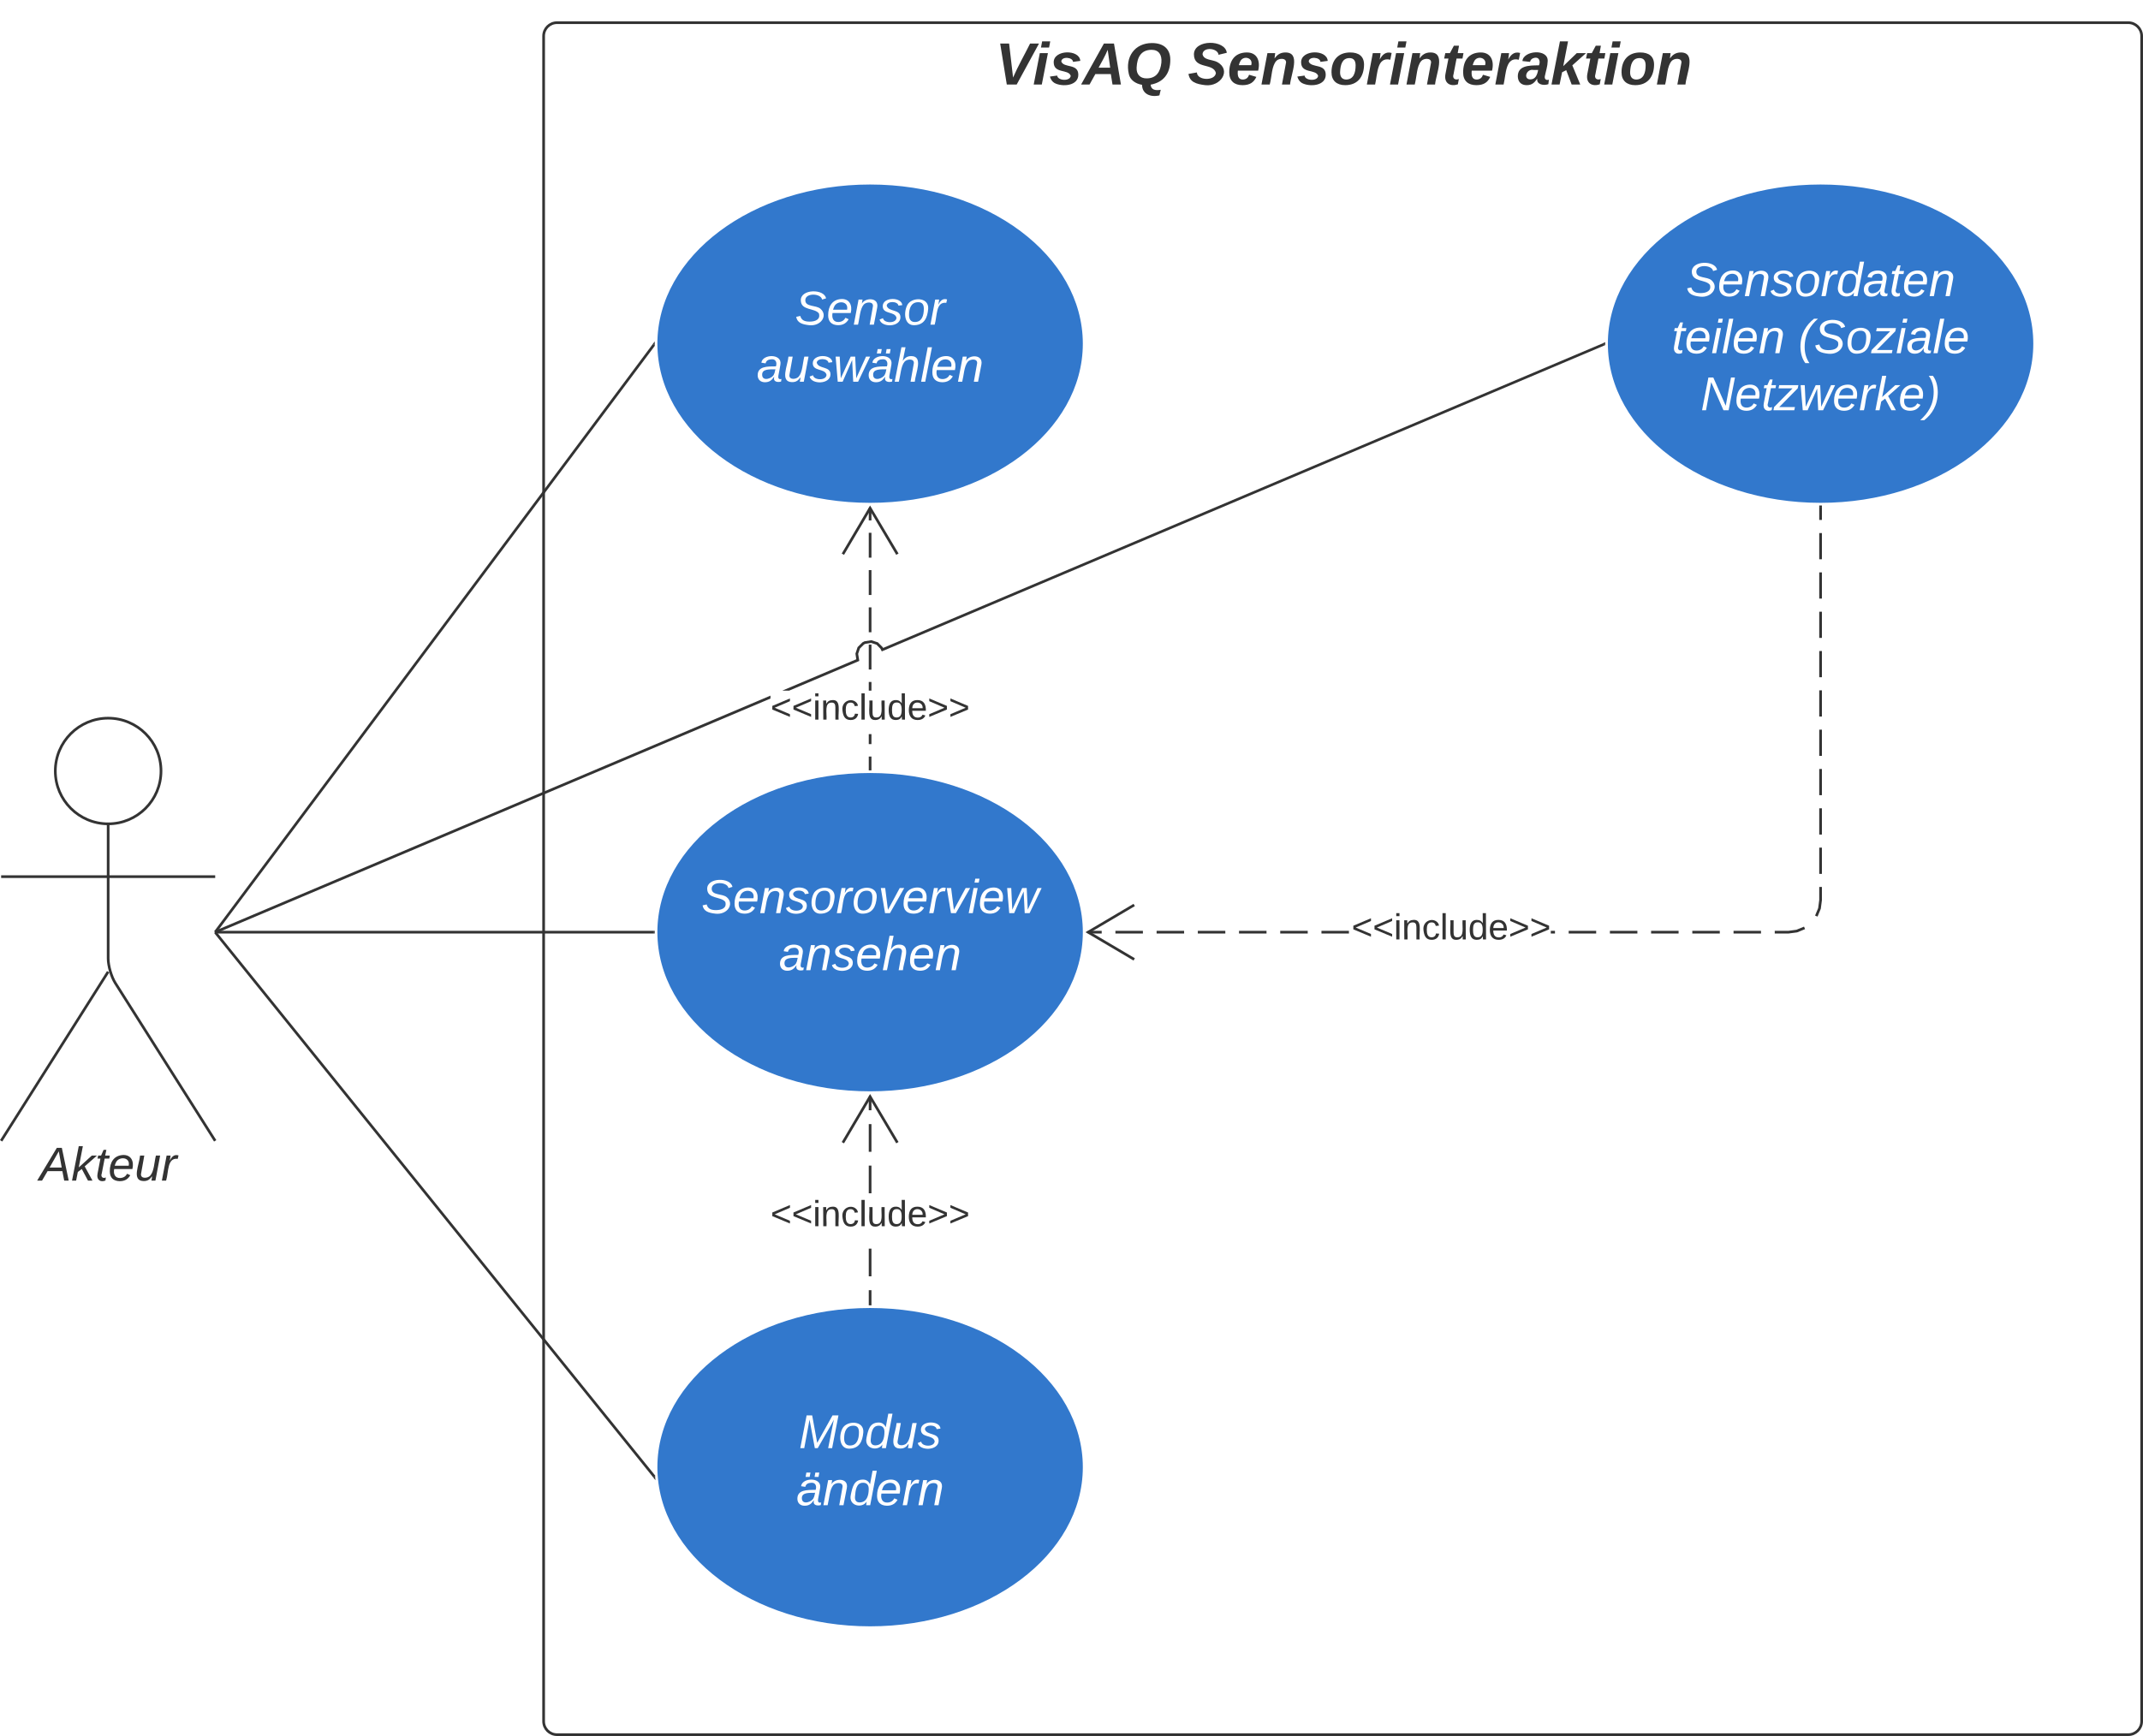
\includegraphics[scale=0.16]{media/activity-usage/Sensorinteraktion}\captionof{figure}{Anwendungsfall für die Interaktionen mit Sensoren} 

\clearpage

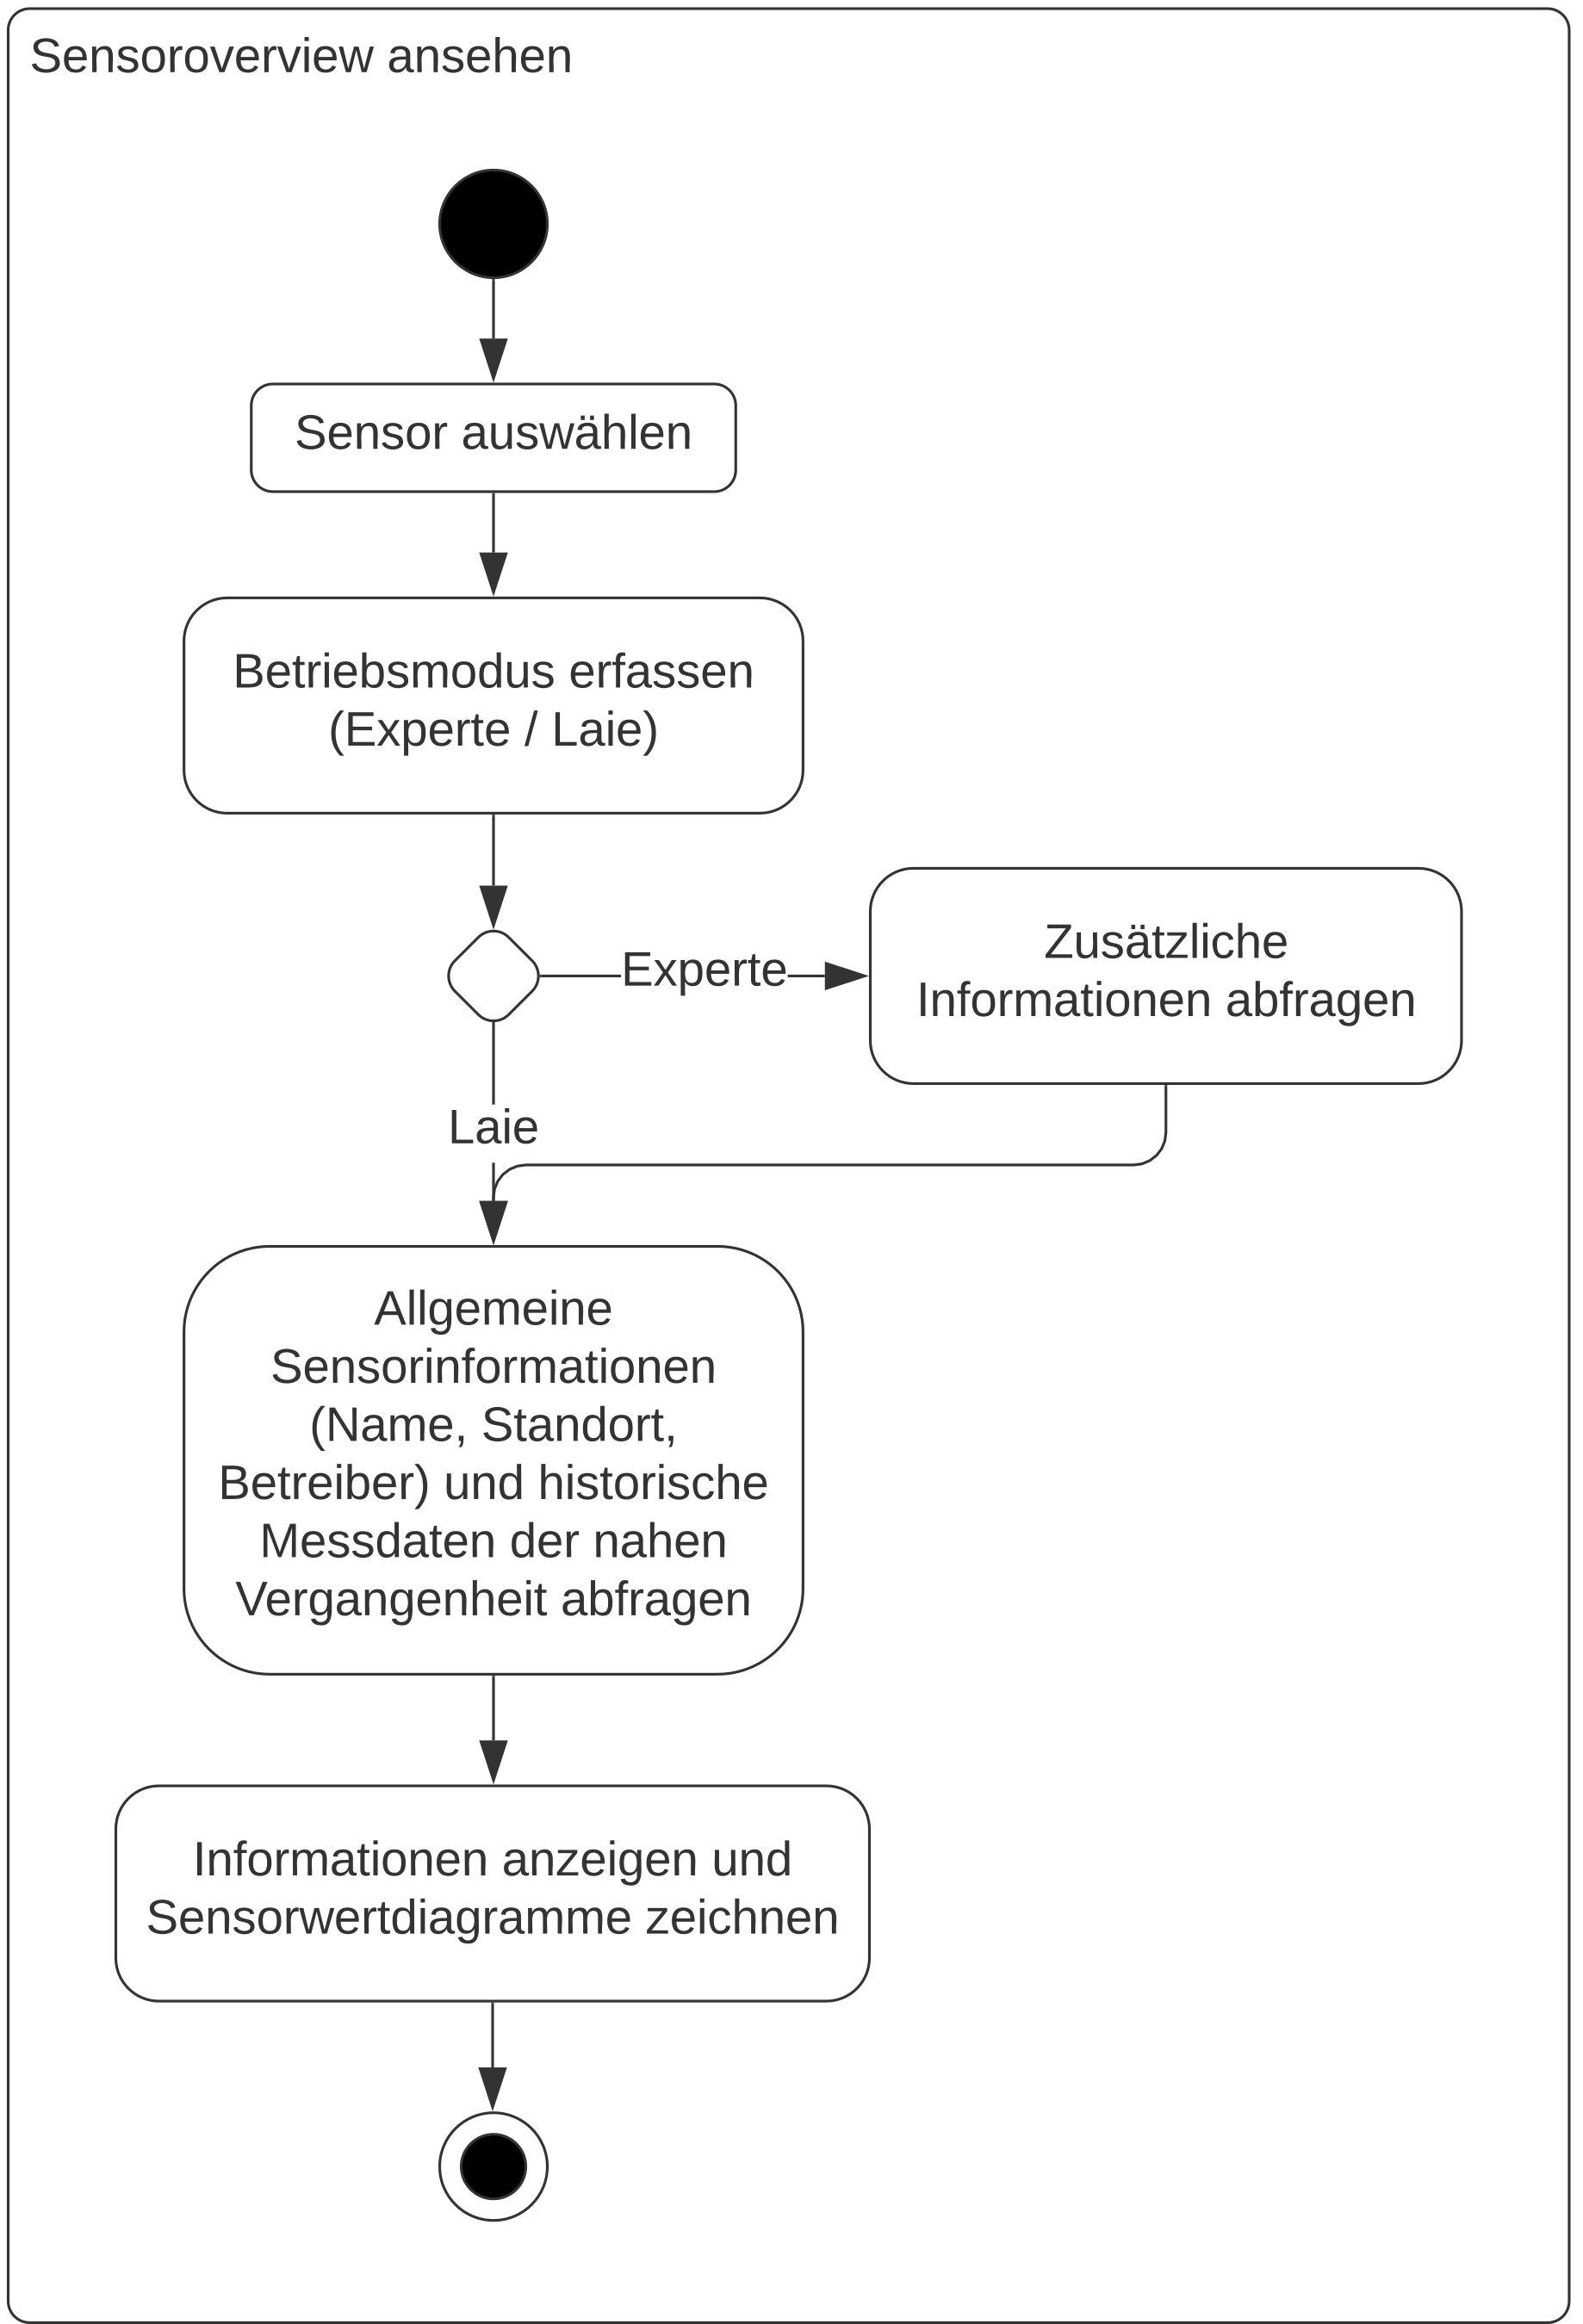
\includegraphics[scale=0.19]{media/activity-usage/SensoroverviewAnsehen}\captionof{figure}{Aufbau der Sensoroverview}
\end{center}